

\begin{figure}[h!]
    \begin{center}
        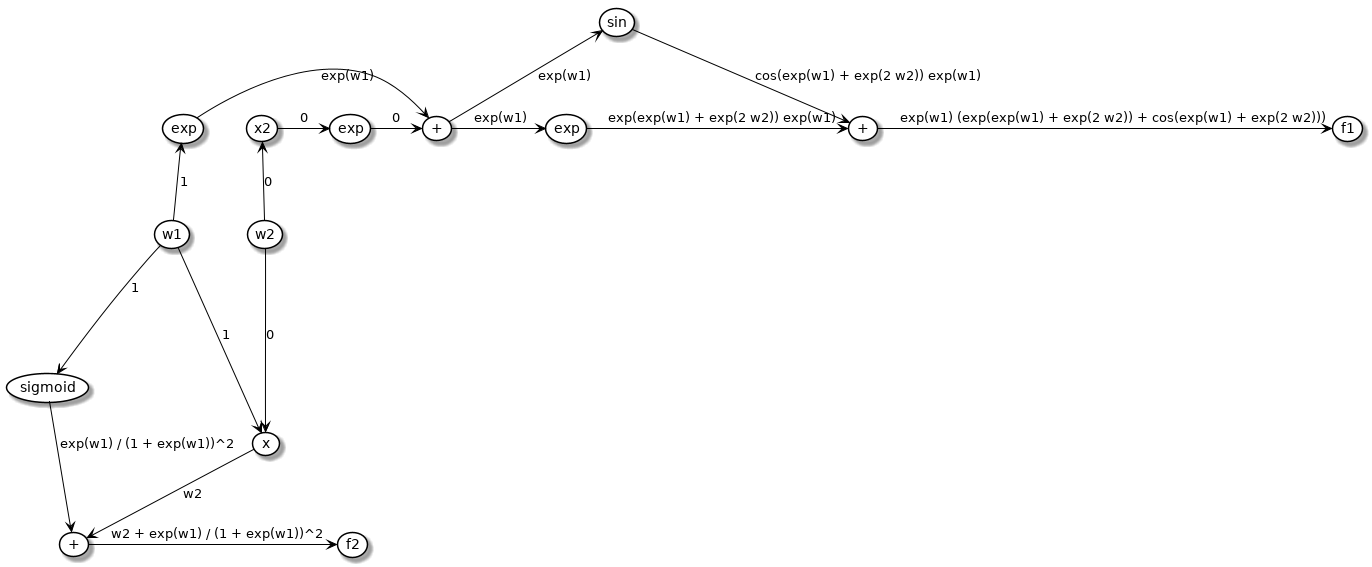
\includegraphics[width=.95\textwidth]{../2_automatocDifferentiation/computation_graph_forward_w1.png}
        \caption{Forward gradient decent on $\vec{f}$ for $w1$}
    \end{center}
\end{figure}

\begin{figure}[h!]
    \begin{center}
        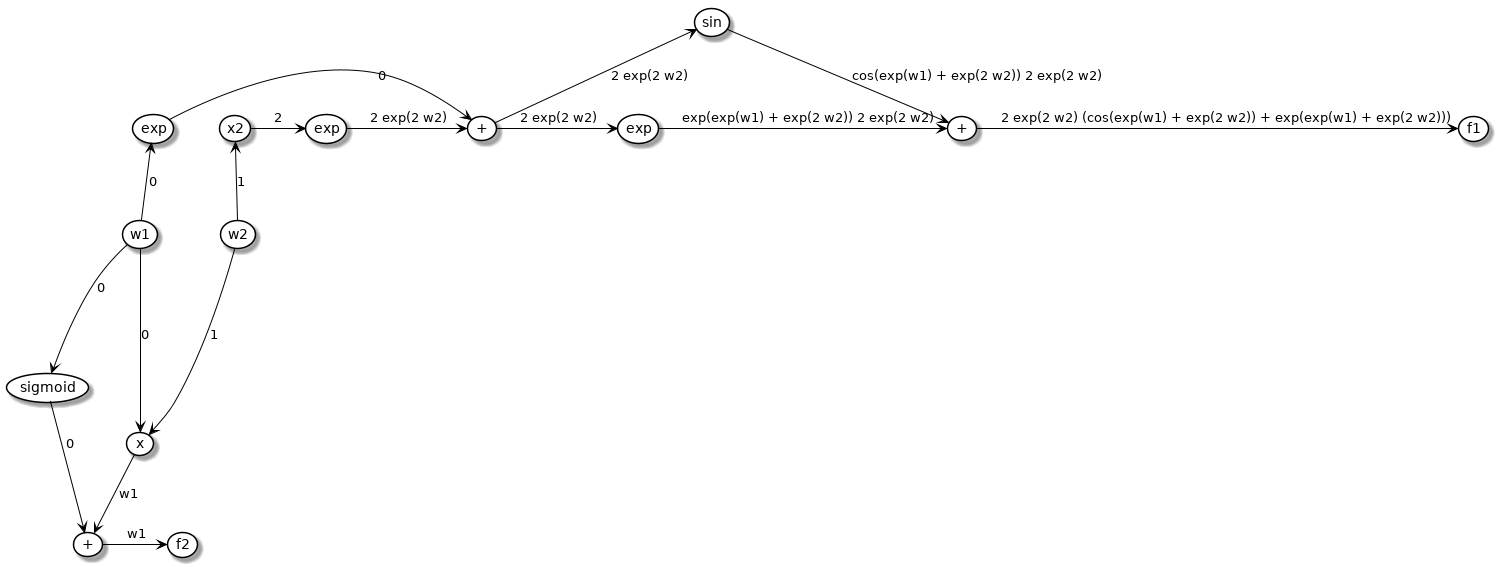
\includegraphics[width=.95\textwidth]{../2_automatocDifferentiation/computation_graph_forward_w2.png}
        \caption{Forward gradient decent on $\vec{f}$ for $w2$}
    \end{center}
\end{figure}

Which in a more mathematical format give us:

\[
    \frac{\partial \vec{f}}{\partial \vec{w}} =
    \begin{bmatrix}
        ( \cos(e^{w_1} + e^{2 w_2}) + e^{e^{w_1} + e^{2 w_2}} ) e^{w_1}   &   2 ( \cos(e^{w_1} + e^{2 w_2}) + e^{e^{w_1} + e^{2 w_2}} ) e^{2 w_2} \\
        \frac{e^{w_1}}{(1 + e^{w_1})^2} + w_2                             &   w_1
    \end{bmatrix}
\]

